\documentclass[12pt]{article}
\usepackage{iftex}
\usepackage{graphicx}
\usepackage{enumitem}
\usepackage{hyperref}
\usepackage[style=apa, backend=biber]{biblatex}
\addbibresource{phd_bombus.bib}
\setcounter{maxnames}{20}
\setcounter{minnames}{1}
\usepackage{color}
\usepackage{amsmath}
\usepackage{amssymb}
\usepackage[export]{adjustbox}
\usepackage{verbatim}
\usepackage{mathpazo}
\usepackage{setspace}
\usepackage{multirow}
\usepackage{lscape}
\usepackage{fancyhdr}
\usepackage[normalem]{ulem}
\usepackage{rotating}
\usepackage{chngcntr}
\usepackage{float}
\usepackage[parfill]{parskip}
\usepackage[tiny,compact]{titlesec}
\usepackage{longtable}
\usepackage{textcomp}
\usepackage{rotating}
\usepackage{xr}
\usepackage{caption}
\usepackage{siunitx}
\usepackage[T1]{fontenc}
\usepackage{gensymb}
\sisetup{round-mode=places, round-precision=2, detect-all}

\newcommand{\flagged}[1] {
  \textcolor{blue}{#1}
}

\hypersetup{colorlinks=true, linkcolor=black, citecolor=black}
\RequirePackage{lineno}

\renewcommand{\thefigure}{A\arabic{figure}}  % Prefix figures with "S"
\setcounter{figure}{0}  % Reset figure counter
\renewcommand{\thetable}{A\arabic{table}}
\setcounter{table}{0}
\setcounter{section}{0}

\def\title{Appendix 1 -- Population Genetics and Colony Assignments}



\begin{document}
\begin{center}
  {\large \title \par}
\end{center}\par

\section{Assessing locus $F_{is}$, $F_{st}$ and linkage disequilibrium}

\begin{figure}[H]
    \centering
    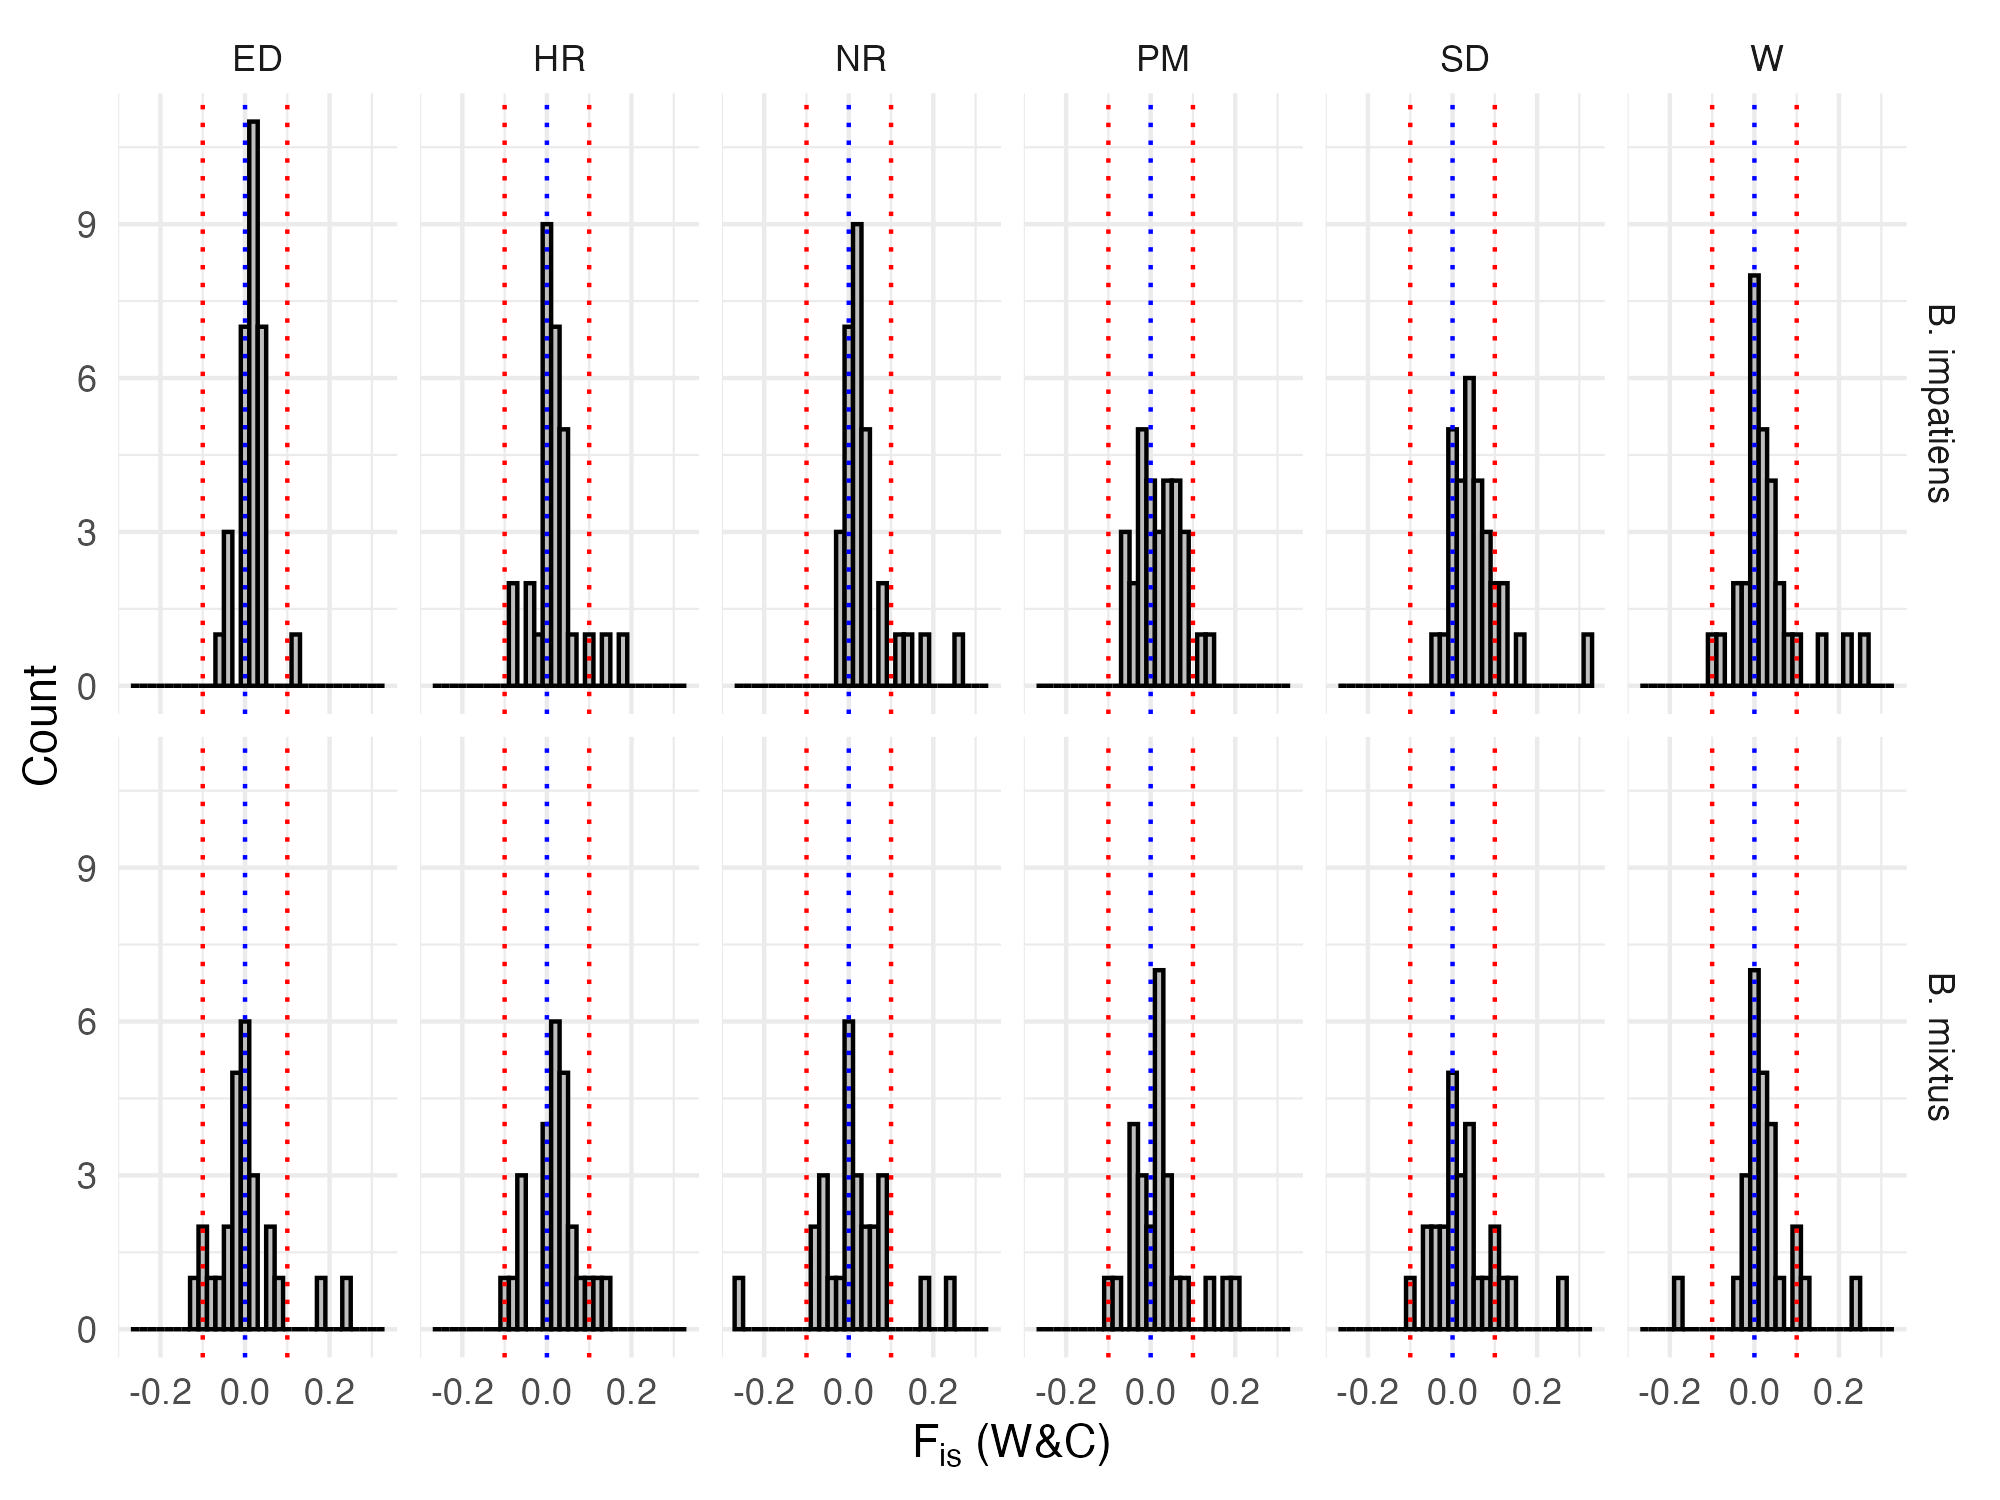
\includegraphics[width=\linewidth]{appendix_figures/Fis.jpg}
    \caption{Estimates of $F_{is}$ for each locus in each subpopulation. Estimates from 2022 and 2023 were calculated separately but are shown together for each site x species combination. Blue dotted lines indicates $F_{is} = 0$ and red dotted lines indicate $F_{is} = \pm 0.1$.}
    \label{fig:Fis}
\end{figure}


\begin{figure}[H]
    \centering
    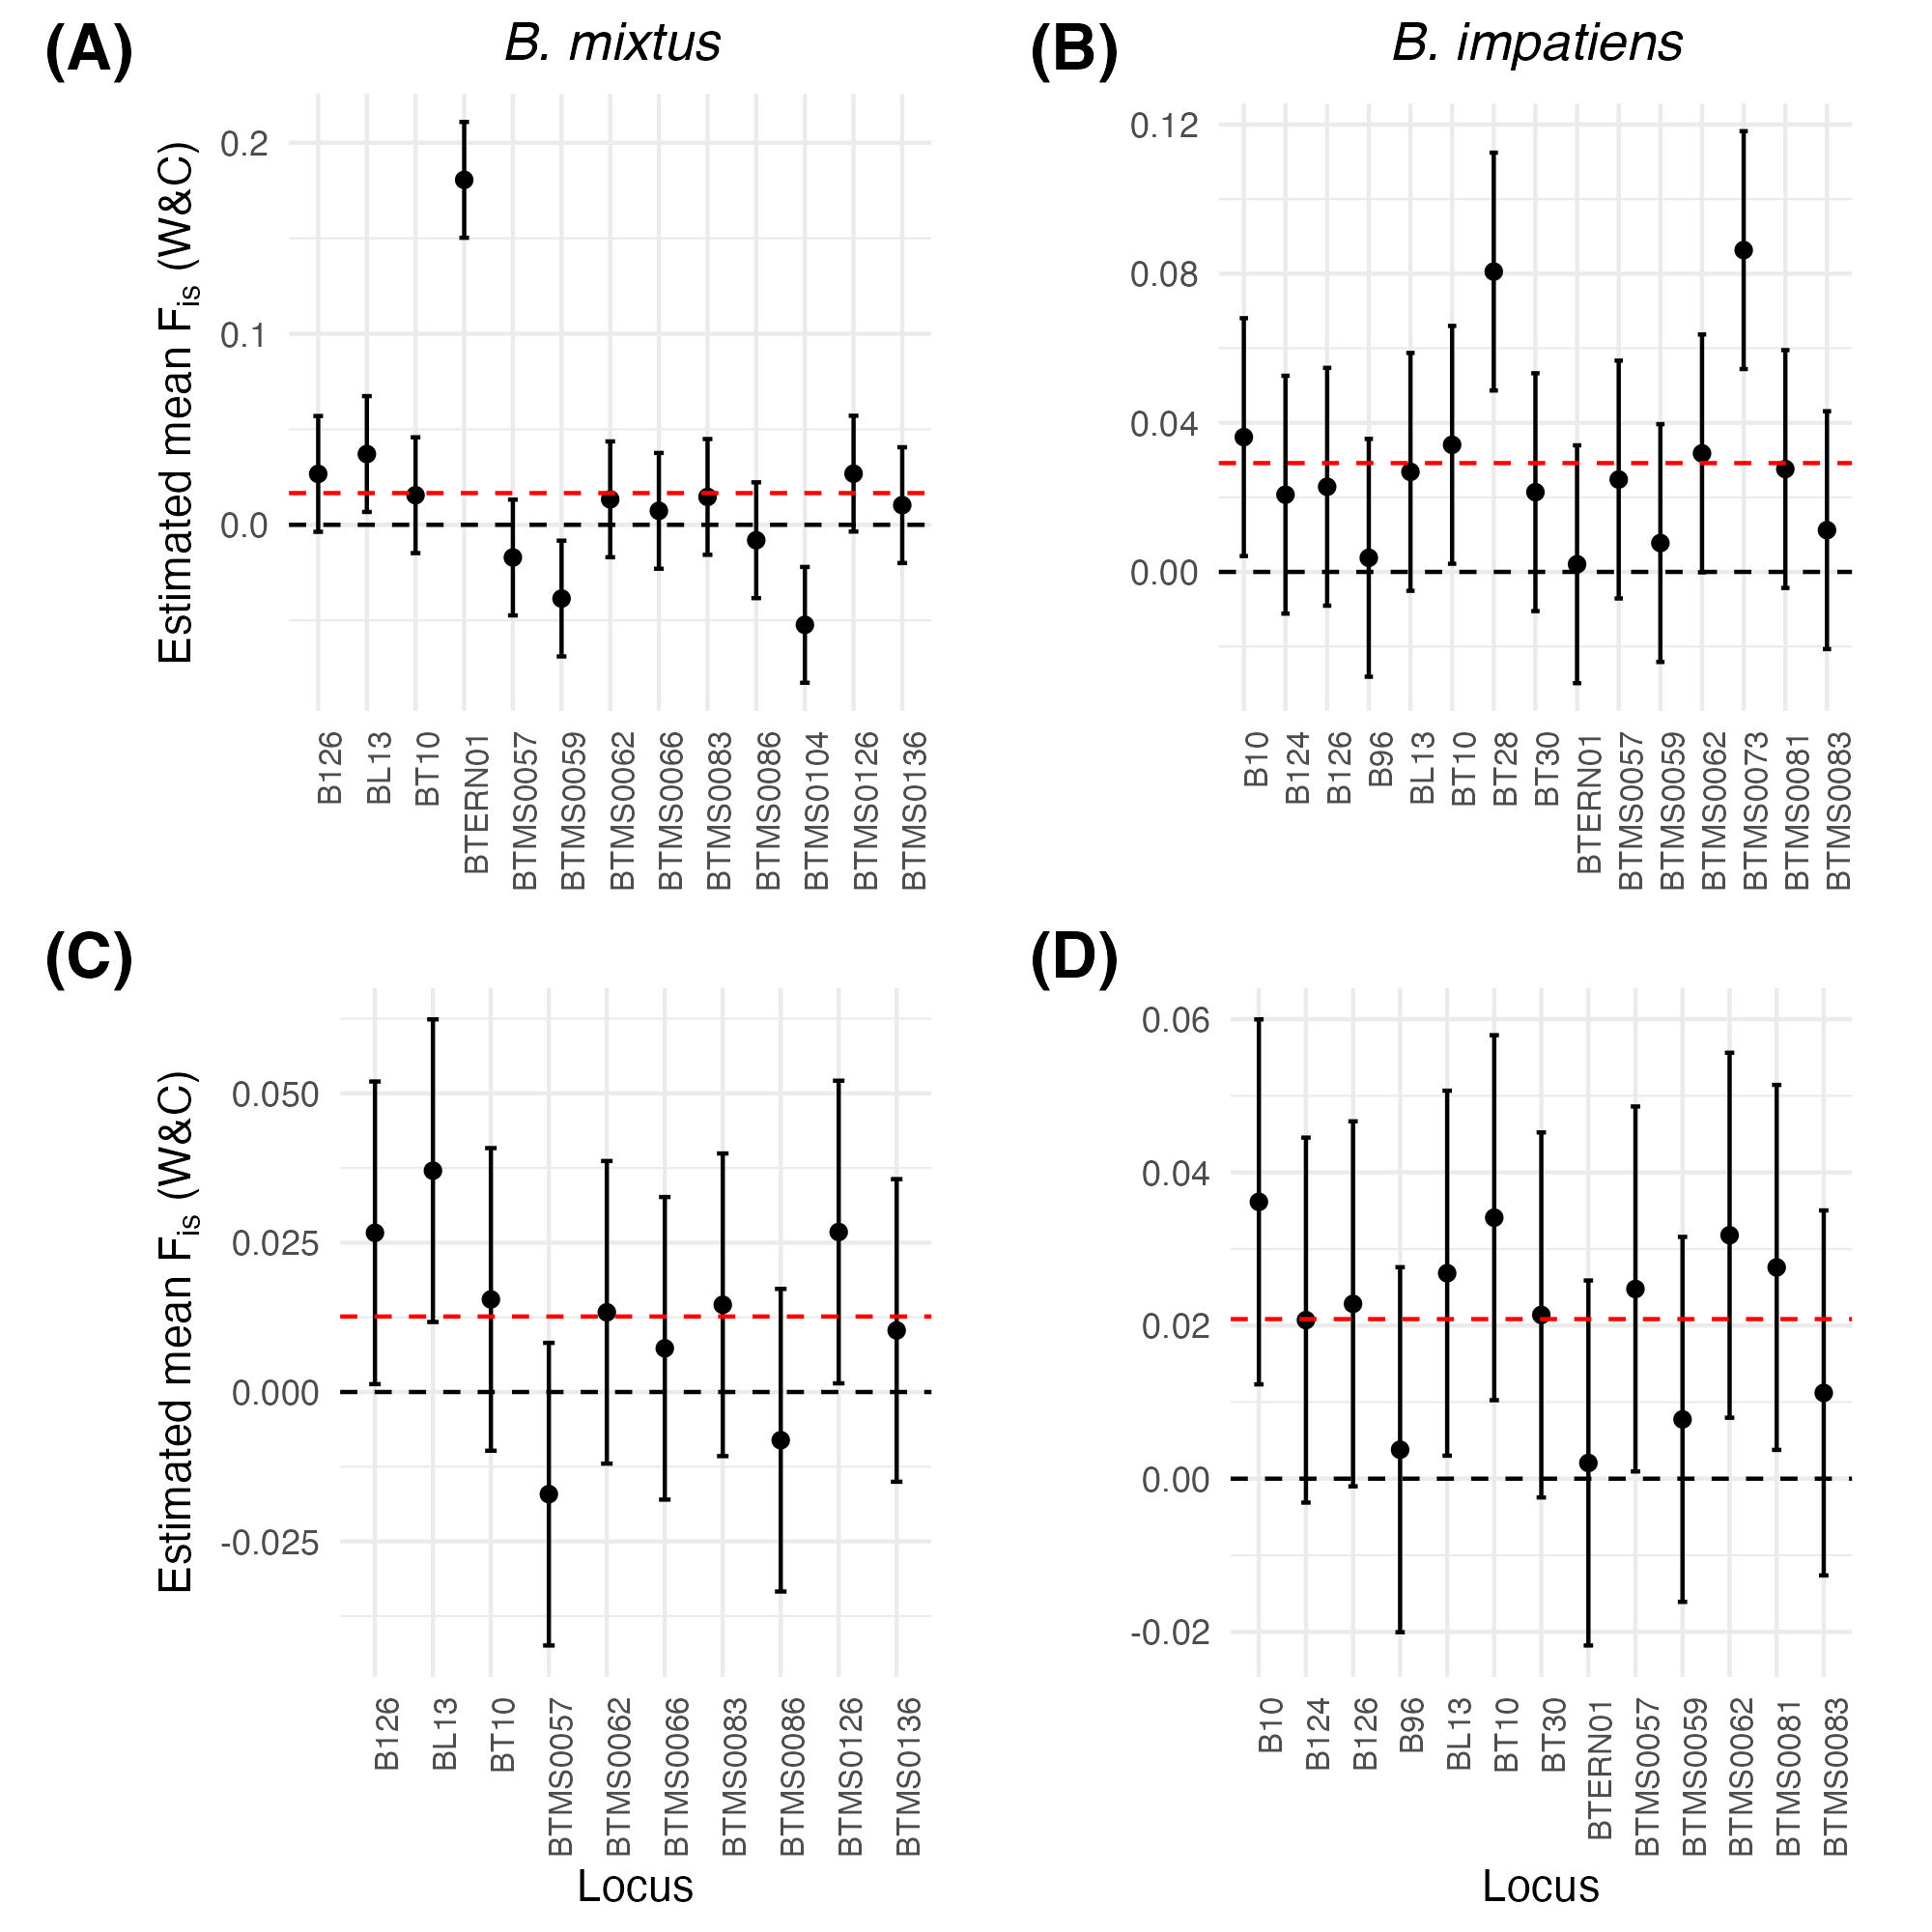
\includegraphics[width=\linewidth]{appendix_figures/marginalmeans.jpg}
    \caption{Locus-specific $F_{is}$ marginal means. A) \emph{B. mixtus} all loci; B) \emph{B. impatiens} all loci; C) \emph{B. mixtus} loci following iterative removal of loci which differed significantly from global mean $F_{is}$; D) \emph{B. impatiens} loci following iterative removal of loci which differed significantly from global mean $F_{is}$. Dashed black line denotes $F_{is} = 0$, dashed red line denotes global mean $F_{is}$ for each species.}
    \label{fig:marginalmeans}
\end{figure}


\begin{figure}[H]
    \centering
    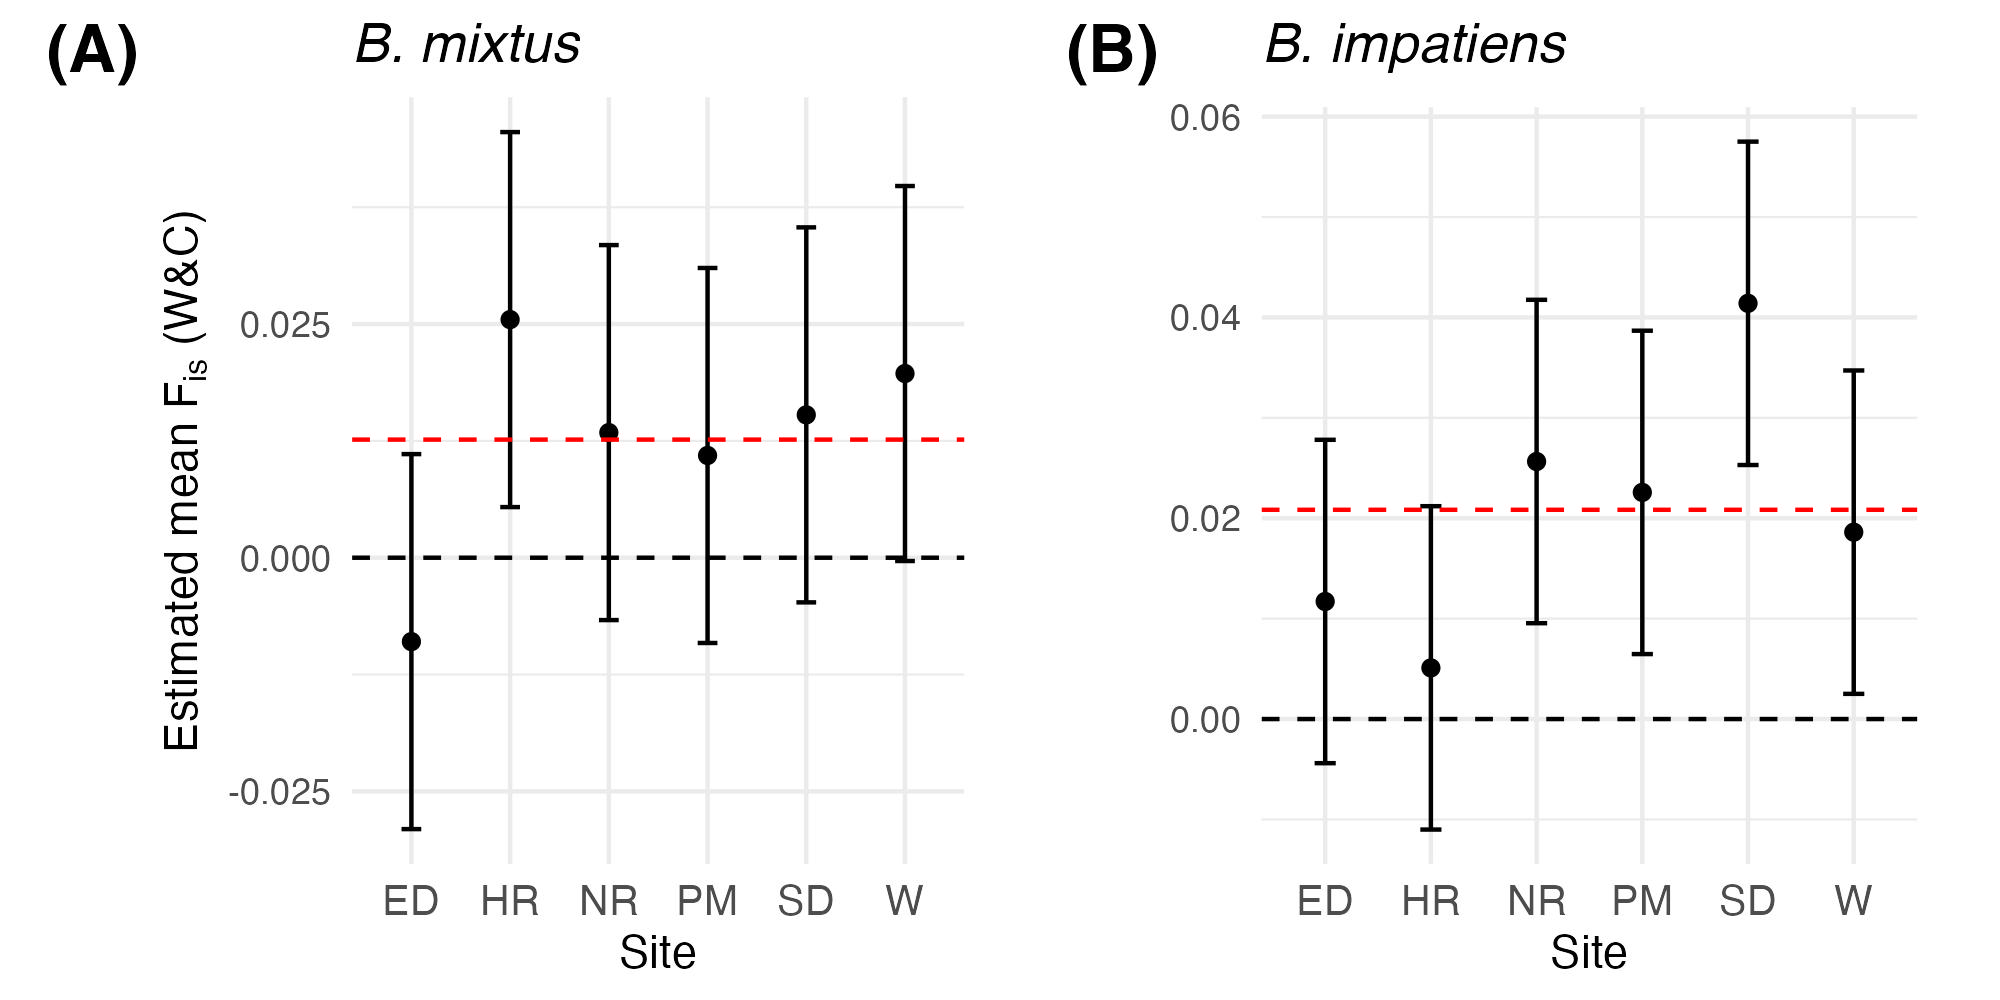
\includegraphics[width=\linewidth]{appendix_figures/siteFis.jpg}
    \caption{Site-specific $F_{is}$ marginal means following removal of low-quality loci for A) \emph{B. mixtus} and B) \emph{B. impatiens}. Dashed black line denotes $F_{is} = 0$, dashed red line denotes global mean $F_{is}$ for each species.}
    \label{fig:siteFis}
\end{figure}


\section{Testing COLONY on simulated data}
To test the informativeness of our genetic loci and to validate the accuracy of COLONY2.0 \parencite{jonesCOLONYProgramParentage2010} for accurately detecting siblingships amongst our samples, we performed simulations using realistic family size distributions and the allelic frequencies present in our real data.

We approached this simulations with four objectives:

(i) To determine false positive and false negative siblingship assignment rates, given the informativeness of our microsatellite datasets, 

(ii) To inform an appropriate strategy (probability threshold, number of runs of the software) for maintaining or rejecting each sib-pair;

(iii) To select suitable software parameters, and in particular to evaluate the usefulness of siblingship size priors and exclusion of across-site siblingships for reducing false positive rates as sample size increases;

(iv) To assess whether modelling female polygamy would improve family reconstruction in the case of sibling genotypes simulated under varying rates of multiple paternity.

\subsection{Simulation strategy}

\subsubsection{Spatially explicit siblingships}
We first simulated spatially explicit siblingships following \textcite{popeInferringForagingRanges2017}. We began by simulating six 5 x 5 trapping grids (locations $k \in \kappa$) on a single raster surface comprised of cells $j \in \mathbb{J}$. Colonies ($i \in \mathbb{C}$) were distributed uniformly at random throughout the ``landscape."

We sampled individuals from colonies $i \in \mathbb{C}$ captured at traps $k \in \mathbb{K}$ from the joint distribution $\Pr(s, c \mid s \in \kappa)$, where $\{s,c\}$ are the indices of a random visitation event of an individual from colony $c \in \mathbb{C}$ to grid cell $s \in \mathbb{J}$.

To do this, we first sampled a trap ($k$) from

\[
\Pr(s = k \mid s \in \kappa) \;=\; \frac{\Pr(s = k)}{\Pr(s \in \kappa)} \tag{1}
\]

where

\[
\Pr(s = k) \;=\; \sum_{i \in C} \Pr(s = k \mid c = i)\,\Pr(c = i)
\]

and

\[
\Pr(s \in \kappa) \;=\; \sum_{i \in \mathbb{C}} \Pr(s \in \kappa \mid c = i)\,\Pr(c = i)
                  \;=\; \sum_{i \in \mathbb{C}} \sum_{k \in \kappa} \Pr(s = k \mid c = i)\,\Pr(c = i)
\]

Combining these statements gives a probability of sampling from trap $k$ of:

\[
\Pr(s = k \mid s \in \kappa) \;=\; \frac{\sum_{i \in C} \Pr(s = k \mid c = i)\,\Pr(c = i)}{\sum_{i \in \mathbb{C}} \sum_{k \in \kappa} \Pr(s = k \mid c = i)\,\Pr(c = i)} \tag{2}
\]

We then sampled a colony ($i$) from

\[
\Pr(c = i \mid s = k) \;=\; \frac{\Pr(s = k \mid c = i) \Pr(c = i)}{\Pr(s = k)} \;=\; \frac{\Pr(s = k \mid c = i) \Pr(c = i)}{\sum_{i \in \mathbb{C}} \Pr(s = k \mid c = i)\,\Pr(c = i)} \tag{3}
\]


We define the foraging kernel of workers from colony $i$ as:

\[
\Pr(s = k \mid c = i)
\;=\; 
\frac{\lambda_i(k)}{\sum_{j \in J} \lambda_i(j)} \tag{4}
\]

The visitation intensity of individuals from colony $i$ to location $j$ is defined as: 

\[
ln(\lambda_i(j)) = \frac{- \lVert x_j - \delta_i \rVert}{\rho} \tag{5}
\]

where $x_j$ are the spatial coordinates of any grid cell in the raster, and $\delta_i$ are the spatial coordinates of colony $i$. The foraging kernel in this example is therefore assumed to be symmetrical and exponentially decaying as a function of distance from the colony location. This means that the total visitation of each colony across the landscape ($\sum_{j \in J} \lambda_i(j)$) is the same for all colonies, and can be represented using the constant $\mathbb{D}$. $\Pr(c = i)$ is the proportion of all bees in the landscape originating from colony $i$, e.g., $\Pr(c = i) = \frac{n_i}{N}$ where $n_i$ is the number of bees from colony $i$, and $N = \sum_{i \in \mathbb{C}} n_i$ is the total number of bees in the landscape.

Combining (4) with (2) and (3) gives the probability of sampling an individual from trap $k$

% with variable foraging kernels
%\[
%\Pr(s = k \mid s \in \kappa) \;=\; \frac{\sum_{i \in \mathbb{C}} \frac{\lambda_i(k)}{\sum_{j \in %J} \lambda_i(j)}\,\frac{n_i}{N}}{\sum_{k \in \kappa} \sum_{i \in \mathbb{C}} \frac{\lambda_i(k%)}{\sum_{j \in J} \lambda_i(j)}\,\frac{n_i}{N}}
%\]

% with identical foraging kernels
\[
\Pr(s = k \mid s \in \kappa) \;=\; \frac{\sum_{i \in \mathbb{C}} \lambda_i(k) \frac{n_i}{N}}{\sum_{k \in \kappa} \sum_{i \in \mathbb{C}} \lambda_i(k) \frac{n_i}{N}}
\]

and the probability that the individual originates from colony $i$

% with variable foraging kernels
% \[
% \Pr(c = i \mid s = k) \;=\;  \frac{\frac{\lambda_i(k)}{\sum_{j \in J} \lambda_i(j)} \frac{n_i}{N}}{\sum_{i \in \mathbb{C}} \frac{\lambda_i(k)}{\sum_{j \in J} \lambda_i(j)} \frac{n_i}{N}}
% \]

% with identical foraging kernels
\[
\Pr(c = i \mid s = k) \;=\; \frac{\lambda_i(k) \frac{n_i}{N}}{\sum_{i \in \mathbb{C}} \lambda_i(k) \frac{n_i}{N}}
\]

For each simulation, samples are drawn from $\Pr(s, c \mid s \in \kappa)$ until a stopping point (desired number of samples) is reached. $n_i$ is updated after each "sampling event" to prevent oversampling from colonies located very close to traps.

To verify that the size of sampled siblingships (e.g., number of siblings per sibling group) accurately mirrors the distribution of siblingship sizes in real data, we compared our simulated distributions to the distribution of siblingshp sizes in our real data (\ref{fig:sibshipsizedist}). For this simulation strategy, we found that moderating the background density of colonies (i.e., the total number of colonies simulated on the landscape) was the most effective strategy for moderating average siblingship size. A larger number of simulated colonies resulted in a higher proportion of singleton colonies (colonies represented by only a single individual).

%%%%%%% INSERT SIBSHIP SIZE DISTRIBUTION FIGURE HERE!!!! %%%%%%%%%%%%%


\subsubsection{Multilocus genotypes}
We simulated multilocus genotypes for each sampled individual under several mating scenarios. In the simplest case, we assume monogamy for both males and queens. The majority of the simulation results presented below follow this assumption. In a second set of simulations, we assumed varying rates of multiple paternity (e.g., queen polygamy) to assess the impact of this assumption on siblingship inferences. For each simulation we used the following heuristic:

(i) Simulate parental genotypes for each siblingship based on the allele frequencies present in our real data;

(ii) Randomly draw offspring genotypes from the set of possible parental alleles at each locus.

We performed simulations based on allele frequencies for both species (\emph{B. mixtus} and \emph{B. impatiens}) because variation in marker number and/or polymorphic information content could lead to differing results. We used inferred allele frequencies from an earlier run of COLONY2.0, which accounts for heightened frequency of alleles present in large families; although raw allele frequencies would have likely been sufficient, given that average family size was small (<2 individuals) and families with > 4 individuals were rare for both datasets.

In the case of monogamous matings, male genotypes were assigned directly to all offspring in the siblingship; in families which were assigned multiple paternity, we assumed two fathers and drew alleles from $\Pr(father_1, father_2) = (0.7, 0.3)$ following the proportions observed for \emph{B. impatiens} in \textcite{birdMatingFrequencyEstimation2024}.

After assigning a multilocus genotype to each individual, we introduced errors and data missingness based on observed error and missingness rates in our real datasets. To introduce errors, we mutated each allele with a probability equal to the rate of errors for that locus and species; we assumed that most errors would be due to contamination, rather than allele dropout, and drew new (erroneous) alleles from the same allele frequencies described above. In the case of data missingness, we observed that individuals which were missing data for \emph{one} copy of a locus were more likely to be missing data for \emph{both} copies than if missingness were distributed uniformly at random. This is likely because there were two primary missingness-generating processes in real data: amplification failure (both alleles missing for an individual) and binning failure (one or both alleles missing for an individual). (In cases were only one copy of a locus failed to amplify, heterozygous individuals would be falsely classified as homozygous---an error, rather than missing data). To account for the structure of missingness, we first calculated the proportion of missing data for each marker ($P_{missing}$) and then removed data for (i) both alleles of each individual with probability $1/3 * P_{missing}$ and for (ii) a single allele per individual with probability $1/3 * P_{missing}$.

\subsection{Determining an appropriate heuristic for maintaining or rejecting inferred siblingships}

It has been previously noted (or speculated) in the literature than COLONY is prone to inferring siblingships between non-siblings, referred to hereafter as \emph{false positive sibships}. Our own preliminary data analyses suggested that this was the case (e.g., a high number of inferred siblingships between individuals separated by >20 km, when individuals from all study sites were permitted to form siblingships). While the biologically of bumblebees does not unilaterally exclude the possibility of such distant relationships, the likelihood of observing such separation distances is extremely small (see discussion below, section "Observing colonymates at multiple sites").

A commonly used strategy to deal with false positives is to repeat multiple "runs" (usually 2-5) of the COLONY software on the same dataset, and maintain family groups which are inferred in all runs at or above some confidence threshhold (usually $P \greq 0.95$, but sometimes $P \greq 0.8$). See, for example, \textcite{carvellMolecularSpatialAnalyses2012, raoBumbleBeeHymenoptera2012, dreierFinescaleSpatialGenetic2014a, geibBumbleBeeNest2015a, carvellBumblebeeFamilyLineage2017a, molaWildfireRevealsTransient2020a}. However, we are not aware of any studies which give support for a particular threshhold probability or number of runs necessary to reach a particular confidence level in assignments, or to achieve a satisfactory balance between false positive siblingships and missed (false negative) siblingships. Indeed, the desireable threshhold is likely to vary as a function of the number and informativeness of markers for a given population.

To overcome these limitations, we tested probability exclusion criteria from $P = 0.95$ to $P = 1$, for 1-5 runs of COLONY version 2.0.6.5. Further, we compared the use of family cluster probabilities (COLONY output file .BestCluster) to full sibling dyad probabilities (COLONY output .FullSibDyad).

We found that....

% give results for prob threshold vs more runs -- determine an appropriate probability threshold!
% probably need to conduct some t tests or lm or something...plus plots!

\subsection{Assessing the use of siblingship size priors and cross-site sibling exclusion for reducing false positive rates}
% SECOND sample size effects -- do exclusion tables help?
% --> rerun some of these but without sibship size prior? for below?

\subsection{Evaluating the effects of multiple paternity on siblingship inference}
% Multiple paternity results




\section{Observing colonymates at multiple sites}


\end{document}